% The generic preamble
\documentclass[10pt,letterpaper,fleqn,titlepage]{article}

% Define packages to use
\usepackage{natbib}
\usepackage[dvips]{graphicx,color}
\usepackage{amsmath,amssymb}
\usepackage{bm}
\usepackage{caption}
\usepackage{xr}
\usepackage{ifthen}
\usepackage[dvipdfm,colorlinks,linkcolor=blue,citecolor=blue,urlcolor=blue]{hyperref}
\usepackage{fancybox}
\usepackage{textcomp}
\usepackage{alltt}
%\usepackage{floatflt}
%\usepackage{svn}


% Redefine default page
\setlength{\textheight}{9in}  % 1" above and below
\setlength{\textwidth}{6.75in}   % 0.5" left and right
\setlength{\oddsidemargin}{-0.25in}

% Redefine default paragraph
\setlength{\parindent}{0pt}
\setlength{\parskip}{1ex plus 0.5ex minus 0.2ex}

% Define caption width and default fonts
\setlength{\captionmargin}{0.5in}
\renewcommand{\captionfont}{\sffamily}
\renewcommand{\captionlabelfont}{\bfseries\sffamily}

% Define commands for super- and subscript in text mode
\newcommand{\superscript}[1]{\ensuremath{^\textrm{#1}}}
\newcommand{\subscript}[1]{\ensuremath{_\textrm{#1}}}

% Derived commands
\newcommand{\invcm}{\textrm{cm\superscript{-1}}}
\newcommand{\micron}{\ensuremath{\mu\textrm{m}}}

\newcommand{\df}{\ensuremath{\delta f}}
\newcommand{\Df}{\ensuremath{\Delta f}}
\newcommand{\dx}{\ensuremath{\delta x}}
\newcommand{\Dx}{\ensuremath{X_{max}}}
\newcommand{\Xeff}{\ensuremath{X_{eff}}}

\newcommand{\water}{\textrm{H\subscript{2}O}}
\newcommand{\carbondioxide}{\textrm{CO\subscript{2}}}
\newcommand{\ozone}{\textrm{O\subscript{3}}}

\newcommand{\taup}[1]{\ensuremath{\tau_{#1}}}
\newcommand{\efftaup}[1]{\ensuremath{\tau_{#1}^{*}}}

\newcommand{\textbfm}[1]{\boldmath\ensuremath{#1}\unboldmath}

\newcommand{\rb}[1]{\raisebox{1.5ex}[0pt]{#1}}

\newcommand{\f}[1]{\texttt{#1}}

% Define how equations are numbered
\numberwithin{equation}{section}
\numberwithin{figure}{section}
\numberwithin{table}{section}

% Define a command for title page author email footnote
\newcommand{\email}[1]
{%
  \renewcommand{\thefootnote}{\alph{footnote}}%
  \footnote{#1}
  \renewcommand{\thefootnote}{\arabic{footnote}}
}

% Define a command to print the Office Note subheading
\newcommand{\notesubheading}[1]
{%
  \ifthenelse{\equal{#1}{}}{}
  { {\Large\bfseries Office Note #1\par}%
    {\scriptsize \sc This is an unreviewed manuscript, primarily intended for informal}\\ 
    {\scriptsize \sc exchange of information among JCSDA researchers\par}%
  }
}

% Redefine the maketitle macro
\makeatletter
\def\docseries#1{\def\@docseries{#1}}
\def\docnumber#1{\def\@docnumber{#1}}
\renewcommand{\maketitle}
{%
  \thispagestyle{empty}
  \vspace*{1in}
  \begin{center}%
     \sffamily
     {\huge\bfseries Joint Center for Satellite Data Assimilation\par}%
     \notesubheading{\@docnumber}
  \end{center}
  \begin{flushleft}%
     \sffamily
     \vspace*{0.5in}
     {\Large\bfseries\ifthenelse{\equal{\@docseries}{}}{}{\@docseries: }\@title\par}%
     \medskip
     {\large\@author\par}%
     \medskip
     {\large\@date\par}%
     \bigskip\hrule\vspace*{2pc}%
  \end{flushleft}%
  \newpage
  \setcounter{footnote}{0}
}
\makeatother
\docseries{}
\docnumber{}


% Define a command for a DRAFT watermark
\usepackage{eso-pic}
\newcommand{\draftwatermark}
{
  \AddToShipoutPicture{%
    \definecolor{lightgray}{gray}{.85}
    \setlength{\unitlength}{1in}
    \put(2.5,3.5){%
      \rotatebox{45}{%
        \resizebox{4in}{1in}{%
          \textsf{\textcolor{lightgray}{DRAFT}}
        }
      }
    }
  }
}




\includeonly{Introduction,Response,Radiative_Transfer,Conclusions,srf.app,dtb.app}

% Definitions for tables
\newcommand{\frequency}[1]{\ensuremath{f_{#1}}}
\newcommand{\bfrequency}[1]{\boldmath\frequency{#1}\unboldmath}
\newcommand{\bdf}[1]{\boldmath\df{#1}\unboldmath}
\newcommand{\sideband}[1]{\ensuremath{df_{#1}}}
\newcommand{\bsideband}[1]{\boldmath\sideband{#1}\unboldmath}
\newcommand{\bdeltaf}{\boldmath\ensuremath{\Delta f}\unboldmath}
\newcommand{\up}[1]{\superscript{#1}}

% Title info
\title{ATMS NPP Spectral Response Function Analysis}
\author{P. van Delst\email{paul.vandelst@noaa.gov},
        D.N. Groff\email{david.groff@noaa.gov}\\JCSDA/EMC/SAIC\\[0.25in]
        W.J. Blackwell\email{wjb@mit.edu}\\Massachusetts Institute of Technology\\[0.25in]
        C.L. Chidester\email{Lynn.Chidester@sdl.usu.edu}\\Space Dynamics Laboratory, Utah State University\\[0.25in]
        G. De Amici\email{giovanni.deamici@ngc.com}\\Northrop Grumman Aerospace Systems\\[0.25in]
        S. Swadley\email{steve.swadley@nrlmry.navy.mil}\\Naval Research Laboratory}
\date{July, 2009}
\docnumber{(unassigned)}
\docseries{CRTM}


%-------------------------------------------------------------------------------
%                            Ze document begins...
%-------------------------------------------------------------------------------
\begin{document}
\maketitle

\draftwatermark

% The front matter
%=================
\thispagestyle{empty}
\vspace*{10cm}
\begin{center}
  {\sffamily\Large\bfseries Change History}
  \begin{table}[htp]
    \centering
    \begin{tabular}{|p{2cm}|p{3cm}|p{8cm}|}
      \hline
      \sffamily\textbf{Date} & \sffamily\textbf{Author} & \sffamily\textbf{Change}\\
      \hline\hline
      2009-07-16 & P. van Delst & Initial release.\\
      \hline
    \end{tabular}
  \end{table}
\end{center}
\clearpage
\pagenumbering{arabic}
\setcounter{page}{1}


% The main matter
%================
\chapter{Introduction}
%=====================


\section{Components}
%===================
\label{sec:components}

The LBLRTM I/O library is constructed around five data constructs, described in table \ref{tab:component_definitions}:
\begin{table}[htp]
  \centering
  \caption{The data constructs of the LBLRTM I/O library}
  \begin{tabular}{p{2.5cm} p{12cm}}
    \hline\\[-0.1cm]
    \sffamily\textbf{Component Name} & \sffamily\textbf{Description} \\
    \hline\hline\\[-0.2cm]
    \texttt{Fhdr}  & The file header construct that is present at the start of each layer of data. \\\\
    \texttt{Phdr}  & This is the panel header construct that is present at the start of each ``chunk'' of data (usually referred to as a ``panel''. See following.) \\\\
    \texttt{Panel} & This construct corresponds to a ``chunk'' of spectral data. An LBLRTM datafile is referred to as being a single- or double-panel file. The former means a single spectral quantity is present (e.g. optical depth), and the latter means that two spectral quantities are present (e.g. radiance and transmittances). \\\\
    \texttt{Layer} & This construct contains spectral data for the entire frequency range of an LBLRTM calculation for a single layer. The concept ``layer'' can correspond to the spectral data for individual atmospheric layers of the input profile, or to the final result for an entire atmosphere. \\\\
    \texttt{File}  & This contruct is true to its name. It corresponds to an entire datafile of data which may consist of a single layer or multiple layers, and for single- or double-panel spectral data. \\
  \hline
  \end{tabular}
  \label{tab:component_definitions}
\end{table}

Each component has a definition module to define the object and some basic methods to manipulate it, and an I/O module to read and write instances of the objects from/to file.

Two components -- the file header and panel header -- are standalone, but the others contain other components, i.e. the panel object contains panel headers; the layer object contains file headers; and the file object contains layers. A schematic illustration of how the actual LBLRTM datafile format relates to the component definitions is shown in figure \ref{fig:lblrtm_format}.

Note, however, that when an LBLRTM file is read, the individual panel ``chunks'' of spectral data are concatenated into a single spectrum. Thus the \Panel{} object itself is only used when reading from an LBLRTM file and is not used in the \File{} or \Layer{} objects.

\begin{figure}[htp]
  \centering
  \input{graphics/lblrtm_format.pstex_t}
  \caption{Schematic illustration of the LBLRTM single- and double-panel datafile format. A datafile can contain one, or multiple, layers of data.}
  \label{fig:lblrtm_format}
\end{figure}



\section{Conventions}
%====================
\label{sec:conventions}
The following are conventions that have been adhered to in the current release of the LBLRTM I/O library. They are guidelines intended to make understanding the code at a glance easier, to provide a recognisable ``look and feel'', and to minimise name space clashes.



\subsection{Naming of Objects and Instances of Objects}
%------------------------------------------------------

The object\footnote{The terms ``derived type'' and ``structure'' can also be used as the code is not yet fully OO - that's for future updates.} naming convention adopted for use in the LBLRTM I/O library is, 

\hspace{0.4cm}\f{LBLRTM\_}\textit{name}\f{\_type} 

where \textit{name} is an identifier for the particular component (e.g. panel header, layer, file, etc as listed in table \ref{tab:component_definitions}). All object type names are suffixed with ``\f{\_type}''. The ``\f{LBLRTM\_}'' prefix is to define a namespace to minimise name clashes. An instance of a object is then referred to via its \textit{name}, or some sort of derivate of its \textit{name}. Some object declarations examples are,

\begin{alltt}
  TYPE(\hyperref[fig:LBLRTM_File_type_structure]{LBLRTM_File_type}) :: sp_file, dp_file
  TYPE(\hyperref[fig:LBLRTM_Layer_type_structure]{LBLRTM_Layer_type}) :: layer\end{alltt}



\subsection{Naming of Definition Modules}
%----------------------------------------

Modules containing object definitions are termed \textit{definition modules}. These modules contain the actual object definitions as well as various utility procedures that operate on the object. The naming convention adopted for definition modules in the LBLRTM I/O library is, 

\hspace{0.4cm}\f{LBLRTM\_}\textit{name}\f{\_Define} 

where all definition module names are suffixed with ``\f{\_Define}''. The actual source code files for these modules have the same name with a ``\f{.f90}'' suffix.



\subsection{Naming of I/O Modules}
%---------------------------------

Modules containing all the object I/O procedures are termed, surprise, surprise, \textit{I/O modules}. These modules contain function to read and write LBLRTM format datafiles. The naming convention adopted for I/O modules in the LBLRTM I/O library is, 

\hspace{0.4cm}\f{LBLRTM\_}\textit{name}\f{\_IO} 

where all I/O module names are suffixed with ``\f{\_IO}''. As with the definition modules, the actual source code files for these modules have the same name with a ``\f{.f90}'' suffix.



\subsection{Standard Definition Module Procedures}
%-------------------------------------------------

The definition modules for the user-accessible objects (for practical purposes just \File, although \Layer, \Fhdr, \Panel, and \Phdr are accessible for now) contain a standard set of procedures for use with the object being defined. The naming convention for these procedures is,

\hspace{0.4cm}\f{LBLRTM\_}\textit{name}\f{\_}\textit{action}

where the available default actions for each procedure are listed in table \ref{tab:definition_module_default_procedures}. This is not an exhaustive list but procedures for the actions listed in table \ref{tab:definition_module_default_procedures} are generally going to be present.

The exception is that the objects with no allocatable components do not have a creation procedure.

\begin{table}[htp]
  \centering
  \caption{Default action procedures available in object definition modules. $^{\dagger}$Procedures not available for the \Fhdr{} and \Phdr{} objects. $^{\ddagger}$Procedure available only for the \Layer{} object.}
  \begin{tabular}{p{2.5cm} p{3.5cm} p{8.5cm}}
    \hline\\[-0.1cm]
    \sffamily\textbf{Action} & \sffamily\textbf{Type} & \sffamily\textbf{Description} \\
    \hline\hline\\[-0.2cm]
    \texttt{OPERATOR(==)}             & Elemental function   & Tests the equality of two structures. \\
    \texttt{OPERATOR(/=)}             & Elemental function   & Tests the inequality of two structures. \\
    \texttt{Associated}$^{\dagger}$   & Elemental function   & Tests if the object components have been allocated. \\
    \texttt{Create}$^{\dagger}$       & Elemental subroutine & Allocates any allocatable object components. \\
    \texttt{Destroy}                  & Elemental subroutine & Reinitialises an object. \\
    \texttt{DefineVersion}            & Subroutine           & Returns the module version information. \\
    \texttt{Frequency}$^{\ddagger}$   & Subroutine           & Compute and return the spectral frequency grid. \\
    \texttt{Inspect}                  & Subroutine           & Displays object contents to \texttt{stdout}. \\
    \texttt{IsValid}                  & Elemental function   & Tests if the object contains valid data. \\
    \texttt{SetValid}                 & Elemental subroutine & Flags the object as containing valid data. \\
  \hline
  \end{tabular}
  \label{tab:definition_module_default_procedures}
\end{table}

\begin{table}[htp]
  \centering
  \caption{Default action procedures available in object I/O modules.}
  \begin{tabular}{p{2.5cm} p{3.5cm} p{8.5cm}}
    \hline\\[-0.1cm]
    \sffamily\textbf{Action} & \sffamily\textbf{Type} & \sffamily\textbf{Description} \\
    \hline\hline\\[-0.2cm]
    \texttt{IOVersion} & Subroutine  & Returns the module version information. \\
    \texttt{Read}      & Function    & Loads an instance of an object with data read from file. \\
    \texttt{Write}     & Function    & Write an instance of an object to file. \\
  \hline
  \end{tabular}
  \label{tab:io_module_default_procedures}
\end{table}

Some examples of these procedure names are,

\begin{alltt}
  \hyperref[sec:LBLRTM_File_Associated_interface]{LBLRTM_File_Associated}
  \hyperref[sec:LBLRTM_File_IsValid_interface]{LBLRTM_File_IsValid}
  \hyperref[sec:LBLRTM_Layer_Destroy_interface]{LBLRTM_Layer_Destroy}
  \hyperref[sec:LBLRTM_Layer_Frequency_interface]{LBLRTM_Layer_Frequency}
  \hyperref[sec:LBLRTM_File_Inspect_interface]{LBLRTM_File_Inspect}\end{alltt}

The relational operators, \f{==} and \f{/=}, are implemented via overloaded \f{Equal} and \f{NotEqual} action procedures respectively, as is shown below for the \File{} structure,

\begin{alltt}
  INTERFACE OPERATOR(==)
    MODULE PROCEDURE LBLRTM_File_Equal
  END INTERFACE OPERATOR(==)

  INTERFACE OPERATOR(/=)
    MODULE PROCEDURE LBLRTM_File_NotEqual
  END INTERFACE OPERATOR(/=)\end{alltt}

For a complete list of the definition and I/O module procedures for use with the available objects, see appendix \ref{app:object_and_interface_definition}.


\section{ATMS Response Data}
%===========================

\subsection{Specified and measured responses}
%--------------------------------------------
The NPP ATMS specified central frequencies, sideband offsets and channel bandwidths, taken from table 9 of reference \cite{CrIS_EDR_ATBD}, are shown in table \ref{tab:atms_fo_sb_and_df}. Also shown are measured bandwidths taken from table 12-1 of reference \cite{ATMS_PFM_CalLog}. No measurements of the central frequencies are readily available \footnote{These values may be available in other ATMS reports, particularly: RE-13680 K/Ka Band Receiver Shelf Verification Report, RE-13658 W Band Receiver Shelf Verification Report, RE-13741 V Band Receiver Shelf Verification Report, and RE-13802 G Band Receiver Shelf Verification Report.}.

\begin{table}[htp]
  \centering
  \begin{tabular}{c c c c c c}
    \hline
                     & \textbf{Central}         & \textbf{Sideband 1}   & \textbf{Sideband 2}   & \textbf{Specified}       & \textbf{Measured} \\
                     & \textbf{Frequency}\up{a} & \textbf{Offset}\up{a} & \textbf{Offset}\up{a} & \textbf{Bandwidth}\up{a} & \textbf{Bandwidth}\up{b} \\
    \textbf{Channel} & \bfrequency{0}           & \bsideband{1}         & \bsideband{2}         & \bdeltaf                 & \bdeltaf      \\
                     & (GHz)                    & (GHz)                 & (GHz)                 & (MHz)                    & (MHz)         \\
    \hline\hline
            1        &  23.800000  & -      & -      & 0.27   & 0.258         \\
            2        &  31.400000  & -      & -      & 0.18   & 0.172         \\
            3        &  50.300000  & -      & -      & 0.18   & 0.173         \\
            4        &  51.760000  & -      & -      & 0.40   & 0.381         \\
            5        &  52.800000  & -      & -      & 0.40   & 0.366         \\
            6        &  53.596000  & 0.115  & -      & 0.17   & 0.1587,0.1648\up{c} \\
            7        &  54.400000  & -      & -      & 0.40   & 0.387         \\
            8        &  54.940000  & -      & -      & 0.40   & 0.387         \\
            9        &  55.500000  & -      & -      & 0.33   & 0.317         \\
           10        &  57.290344  & -      & -      & 0.33   & 0.151         \\
           11        &  57.290344  & 0.217  & -      & 0.078  & 0.0763        \\
           12        &  57.290344  & 0.3222 & 0.048  & 0.036  & 0.0351        \\
           13        &  57.290344  & 0.3222 & 0.022  & 0.016  & 0.01547       \\
           14        &  57.290344  & 0.3222 & 0.010  & 0.008  & 0.0078,0.0079\up{c} \\
           15        &  57.290344  & 0.3222 & 0.0045 & 0.003  & 0.0029        \\
           16        &  88.200000  & -      & -      & 2.0    & 1.9282        \\
           17        & 165.500000  & -      & -      & 3.0    & 1.1251        \\
           18        & 183.310000  & 7.0    & -      & 2.0    & 1.9302        \\
           19        & 183.310000  & 4.5    & -      & 2.0    & 1.9519        \\
           20        & 183.310000  & 3.0    & -      & 1.0    & 0.9799        \\
           21        & 183.310000  & 1.8    & -      & 1.0    & 0.9823        \\
           22        & 183.310000  & 1.0    & -      & 0.5    & 0.4940        \\
    \hline
  \end{tabular}
  \caption{Central, sideband offset, and bandwidth frequencies for ATMS. \superscript{a}Data from table 9 of ref.\cite{CrIS_EDR_ATBD}. \superscript{b}Data from table 12-1 of ref.\cite{ATMS_PFM_CalLog}. \superscript{c}Different lower and upper sideband widths reported. }
  \label{tab:atms_fo_sb_and_df}
\end{table}

In addition to the usual frequency parameters, the ATMS PFM Calibration Log \cite{ATMS_PFM_CalLog} contains tables (12-2a to 12-2d) of the digitised filter responses (hereafter referred to as the spectral response functions, or SRFs). Apart from channels 1 and 2, these digitised SRFs are at the intermediate frequencies (IF) at which the measurements were made, not at the actual on-orbit channel frequencies. So, these IF SRFs need to be processed so as to represent the SRFs at the frequencies corresponding to the on-orbit channel radiance measurements. The procedures used to do this for the ``Table 12'' IF SRF are shown schemtatically in figure \ref{fig:r_and_s}. Two operations are performed: translation and reflection; how they are carried out depends on the ATMS channel:

\begin{figure}[htp]
  \centering
  \input{graphics/schematics/r_and_s.pstex_t}
  \caption{Schematic illustration of how the ATMS responses, measured at intermediate frequencies, were processed to SRFs at the measurement frequencies. \textbf{(a)} Single passband channels (3-5, 7-10, 16, 17). \textbf{(b)} Double passband channels (11, 18-22). \textbf{(c)} Quadruple passband channels (12-15). \textbf{(d)} Channel 6.}
  \label{fig:r_and_s}
\end{figure}

\begin{description}
  \item[Single Passband Channels, fig.\ref{fig:r_and_s}(a).] Channels 3-5,7-10,16,17. The measured IF SRFs are simply translated to the channel central frequency, $f_0$. The value of the IF central frequency, $f_{i,0}$, is obtained from the first moment of the SRF.
  \item[Double Sideband Channels, fig.\ref{fig:r_and_s}(b).] Channels 11, 18-22. Here a single measured IF sideband is reflected about 0GHz (corresponding to $f_{i,0}$ in this case) and the two sidebands are then translated to the channel central frequency, $f_0$.
  \item[Quadruple Sideband Channels, fig.\ref{fig:r_and_s}(c).] Channels 12-15. In this case two non-contiguous sidebands are reflected about 0GHz (again, corresponding to $f_{i,0}$) and all four sidebands are then translated to the channel central frequency. 
  \item[Channel 6, fig.\ref{fig:r_and_s}(d).] This channel is mentioned separately since, while it is a double sideband channel, unlike the other double sideband channels the IF SRF data contains the contiguous measurement of both sidebands. Thus only translation is applied to the IR SRF. As with the single passband channels, the IF central frequency is the first moment of the SRF. Note that this leads to a different bandwidth for the two sidebands; a situation one doesn't get for for the typical case in fig. \ref{fig:r_and_s}(b). It does beg the question as to why the same procedure wasn't performed for the other multi-band channels.
\end{description}

A selection of four channels from the Table 12 ATMS SRF data, compared to the boxcar reponse, are shown in figure \ref{fig:srf_selection}. All of the channel SRF are shown in appendix \ref{app:srf}. Two channels were selected for display in figure \ref{fig:srf_selection} to highlight their significant difference from the boxcar response: channel 10 (fig.\ref{fig:srf_selection}(b)) because the spec. bandwidth is quite different from that measured by about a factor of two\footnote{Channel 17 suffers similarly; see figure \ref{fig:atms_npp.ch17.srf}}; and channel 19 (fig.\ref{fig:srf_selection}(d)) because, while the measured data does cover the specified bandwidth, the in-band SRF magnitudes appear to decrease anomalously.

\begin{figure}[htp]
  \centering
  \begin{tabular}{c c}
    \textsf{\textbf{(a)} Channel 6} &
    \textsf{\textbf{(b)} Channel 10} \\
    \includegraphics[scale=0.5]{graphics/srf/atms_npp.ch6.srf.eps} &
    \includegraphics[scale=0.5]{graphics/srf/atms_npp.ch10.srf.eps} \\\\

    \textsf{\textbf{(c)} Channel 11} &
    \textsf{\textbf{(d)} Channel 19} \\
    \includegraphics[scale=0.5]{graphics/srf/atms_npp.ch11.srf.eps} &
    \includegraphics[scale=0.5]{graphics/srf/atms_npp.ch19.srf.eps}
  \end{tabular}
  \caption{Selection of NPP ATMS Table 12 SRF data from reference \cite{ATMS_PFM_CalLog} with the corresponding boxcar response based on table \ref{tab:atms_fo_sb_and_df} data.}
  \label{fig:srf_selection}
\end{figure}




\subsection{Additional Digitised Responses}
%------------------------------------------
After a recent SOAT meeting\footnote{Sounding Operational Algorithm Team (SOAT) Meeting, CrIS/ATMS Cal/Val Team, Integrated Program Office, Silver Spring, Maryland, USA, 20-21 May 2009} where the NPP ATMS Table 12 SRF data was discussed, two of us (Chidester, SDL; and DeAmici, NGAS) separately digitised the graphical SRFs displayed in the ATMS PFM Calibration Data Book\cite{ATMS_PFM_CalLog}. The SDL dataset consisted of channels 1, 12, 13, 14, and 15; and the NGAS dataset consisted of channels 4, 5, 9, 13, and 14. These digitised SRFs, along with the corresponding boxcar and Table 12 SRFs, are shown in figures \ref{fig:sp_digitised_srfs} (single passband channels) and \ref{fig:qp_digitised_srfs} (quadruple passband channels).

\begin{figure}[htp]
  \centering
  \begin{tabular}{c c}
    \textsf{\textbf{(a)} Channel 1} &
    \textsf{\textbf{(b)} Channel 4} \\
    \includegraphics[scale=0.5]{graphics/srf/atms_npp.ch1.srf.eps} &
    \includegraphics[scale=0.5]{graphics/srf/atms_npp.ch4.srf.eps} \\\\

    \textsf{\textbf{(c)} Channel 5} &
    \textsf{\textbf{(d)} Channel 9} \\
    \includegraphics[scale=0.5]{graphics/srf/atms_npp.ch5.srf.eps} &
    \includegraphics[scale=0.5]{graphics/srf/atms_npp.ch9.srf.eps}
  \end{tabular}
  % the hand-crafted legend
  \setlength{\unitlength}{1cm}
  \begin{picture}(2.0,2.0)
    \thicklines
    \color{blue}
    \put(0.0,0.2 ){\line(1,0){1}}
    \put(1.1,0.05){\sffamily NGAS}
    \color{green}
    \put(0.0,0.7 ){\line(1,0){1}}
    \put(1.1,0.55){\sffamily SDL}
    \color{red}
    \put(0.0,1.2 ){\line(1,0){1}}
    \put(1.1,1.05){\sffamily Table 12}
    \color{black}
    \put(0.0,1.7 ){\line(1,0){1}}
    \put(1.1,1.55){\sffamily Boxcar}
  \end{picture}
  \caption{Single passband SDL and NGAS digitised NPP ATMS SRFs from reference \cite{ATMS_PFM_CalLog} with the corresponding boxcar and Table 12 response}
  \label{fig:sp_digitised_srfs}
\end{figure}

For the single passband channels shown in figure \ref{fig:sp_digitised_srfs}, the SDL channel 1 digitisation of fig.\ref{fig:sp_digitised_srfs}(a) appears to be most like the Table 12 representation. For the NGAS digitisations, figs.\ref{fig:sp_digitised_srfs}(b)-(d), the outstanding feature is how very different the digitised data is from the Table 12 data. Lest readers think the digitisation procedures somehow went awry, they are referred to Appendix \ref{app:srf} -- in particular figures \ref{fig:atms_npp.ch1.srf}, \ref{fig:atms_npp.ch4.srf}, \ref{fig:atms_npp.ch5.srf}, and \ref{fig:atms_npp.ch9.srf} -- where the plots shown in \ref{fig:sp_digitised_srfs} are replicated at a larger size, but also with the corresponding filter response taken from the ATMS PFM Calibration Data Book \cite{ATMS_PFM_CalLog}. Comparison of these plots clearly show that the SDL and NGAS digitisations are more respresentative of the measurements displayed in \cite{ATMS_PFM_CalLog}.

\begin{figure}[htp]
  \centering
  \begin{tabular}{c c}
    \textsf{\textbf{(a)} Channel 12} &
    \textsf{\textbf{(b)} Channel 13} \\
    \includegraphics[scale=0.5]{graphics/srf/atms_npp.ch12.srf.eps} &
    \includegraphics[scale=0.5]{graphics/srf/atms_npp.ch13.srf.eps} \\\\

    \textsf{\textbf{(c)} Channel 14} &
    \textsf{\textbf{(d)} Channel 15} \\
    \includegraphics[scale=0.5]{graphics/srf/atms_npp.ch14.srf.eps} &
    \includegraphics[scale=0.5]{graphics/srf/atms_npp.ch15.srf.eps}
  \end{tabular}
  % the hand-crafted legend
  \setlength{\unitlength}{1cm}
  \begin{picture}(2.0,2.0)
    \thicklines
    \color{blue}
    \put(0.0,0.2 ){\line(1,0){1}}
    \put(1.1,0.05){\sffamily NGAS}
    \color{green}
    \put(0.0,0.7 ){\line(1,0){1}}
    \put(1.1,0.55){\sffamily SDL}
    \color{red}
    \put(0.0,1.2 ){\line(1,0){1}}
    \put(1.1,1.05){\sffamily Table 12}
    \color{black}
    \put(0.0,1.7 ){\line(1,0){1}}
    \put(1.1,1.55){\sffamily Boxcar}
  \end{picture}
  \caption{Quadruple passband SDL and NGAS digitised NPP ATMS SRFs from reference \cite{ATMS_PFM_CalLog} with the corresponding boxcar and Table 12 response}
  \label{fig:qp_digitised_srfs}
\end{figure}

Similarly, for the quadruple passband channels shown in figure \ref{fig:qp_digitised_srfs}, the SDL and NGAS digitisations are quite different from the Table 12 data. Of particular interest is the difference in relative magnitudes between the ``inner'' (\#2 and \#3) and ``outer'' (\#1 and \#4) bands for channels 13 and 14 in figs.\ref{fig:qp_digitised_srfs}(b) and (c). Comparison of the digitised data with that displayed in the ATMS PFM Calibration Data Book \cite{ATMS_PFM_CalLog} -- see figures \ref{fig:atms_npp.ch12.srf}, \ref{fig:atms_npp.ch13.srf}, \ref{fig:atms_npp.ch14.srf}, and \ref{fig:atms_npp.ch14.srf} -- again shows the SDL and NGAS digitisation to be more respresentative of the filter responses, in both shape and relative magnitude, than the Table 12 data. It should be pointed out that the vertical excursions for the relative response plots are more pronounced than for those where the y-axis is signal loss with units of decibels.
 


\section{Radiative Transfer Calculations}
%========================================
\label{sec:rt}
\subsection{Methodology}
%-----------------------
Monochromatic radiative transfer calculations were done at the various tabulated ATMS SRF frequencies using MonoRTM \cite{Payne_2008,Clough_2005} and the ECMWF83 profile set \cite{Matricardi_ECMWF564,ECMWF_profile_set2}. The subsequent spectra were then convolved with the tabulated SRFs using a simple numerical integration routine.

The temperature and water vapour from the ECMWF83 set are shown in figure \ref{fig:ECMWF83.AtmProfile} to provide an indication of the range of inputs. We realise 83 profiles is a small sample and are looking at repeating the calculations for a larger (1000's of profiles) data set. 

\begin{figure}[htp]
  \centering
  \includegraphics[scale=1]{graphics/atmprofile/ECMWF83.AtmProfile.eps}
  \caption{The temperature and water vapour profiles from the ECMWF83 profile dataset used in the radiative transfer calculations.}
  \label{fig:ECMWF83.AtmProfile}
\end{figure}


\subsection{Results}
%-------------------
The results for the different digitised, or measured, SRFs are presented here as brightness temperature differences from the boxcar SRF result, that is,
\begin{equation}
  \Delta T_B = T_{B,Boxcar} - T_{B,Measured}
\end{equation}
The $\Delta T_B$ values are displayed as a function of $T_{B,Boxcar}$ as well as a histogram of the differences. Only the results for those channels for which we have either SDL or NGAS digistised SRFs will be discussed here. Results for all the channels are shown in Appendix \ref{app:dtb}. Since the reference for the brightness temperatures differences is the boxcar SRF, it should also be noted that these comparisons are intended to highlight the impact of the differences between the various digitised SRFs, not necessarily to indicate which is ``better''.

\subsubsection{Single passband channels: 1, 4, 5, amd 9}
%......................................................
The $\Delta T_B$ scatterplots for the single passband channels 1, 4, 5, and 9 are shown in figure \ref{fig:sp_digitised_dtbs_scatter}, and the corresponding histograms are shown in figure \ref{fig:sp_digitised_dtbs_hist}. In all cases the SDL and NGAS digitisations decreased the $\Delta T_B$ values, although to different degrees.

\begin{figure}[htp]
  \centering
  \begin{tabular}{c c}
    \textsf{\textbf{(a)} Channel 1} &
    \textsf{\textbf{(b)} Channel 4} \\
    \includegraphics[bb=82 289 312 493,clip,scale=1.0]{graphics/dtb/atms_npp.ch1.TbStats.eps} &
    \includegraphics[bb=82 289 312 493,clip,scale=1.0]{graphics/dtb/atms_npp.ch4.TbStats.eps} \\\\

    \textsf{\textbf{(c)} Channel 5} &
    \textsf{\textbf{(d)} Channel 9} \\
    \includegraphics[bb=82 289 312 493,clip,scale=1.0]{graphics/dtb/atms_npp.ch5.TbStats.eps} &
    \includegraphics[bb=82 289 312 493,clip,scale=1.0]{graphics/dtb/atms_npp.ch9.TbStats.eps}
  \end{tabular}
  % the hand-crafted legend
  \setlength{\unitlength}{1cm}
  \begin{picture}(2.0,1.25)(0.0,0.45)
    \thicklines
    \color{blue}
    \put(0.0,0.7 ){\line(1,0){1}}
    \put(1.1,0.55){\sffamily NGAS}
    \color{green}
    \put(0.0,1.2 ){\line(1,0){1}}
    \put(1.1,1.05){\sffamily SDL}
    \color{red}
    \put(0.0,1.7 ){\line(1,0){1}}
    \put(1.1,1.55){\sffamily Table 12}
  \end{picture}
  \caption{Scatterplots of the calculated brightness temperature differences, $\Delta T_B$, as a function of the boxcar SRF $T_{B,Boxcar}$ for the single passband SDL and NGAS digitised SRFs}
  \label{fig:sp_digitised_dtbs_scatter}
\end{figure}

\begin{figure}[htp]
  \centering
  \begin{tabular}{c c}
    \textsf{\textbf{(a)} Channel 1} &
    \textsf{\textbf{(b)} Channel 4} \\
    \includegraphics[bb=312 289 538 493,clip,scale=1.0]{graphics/dtb/atms_npp.ch1.TbStats.eps} &
    \includegraphics[bb=312 289 538 493,clip,scale=1.0]{graphics/dtb/atms_npp.ch4.TbStats.eps} \\\\

    \textsf{\textbf{(c)} Channel 5} &
    \textsf{\textbf{(d)} Channel 9} \\
    \includegraphics[bb=312 289 538 493,clip,scale=1.0]{graphics/dtb/atms_npp.ch5.TbStats.eps} &
    \includegraphics[bb=312 289 538 493,clip,scale=1.0]{graphics/dtb/atms_npp.ch9.TbStats.eps}
  \end{tabular}
  % the hand-crafted legend
  \setlength{\unitlength}{1cm}
  \begin{picture}(2.0,1.25)(0.0,0.45)
    \thicklines
    \color{blue}
    \put(0.0,0.7 ){\line(1,0){1}}
    \put(1.1,0.55){\sffamily NGAS}
    \color{green}
    \put(0.0,1.2 ){\line(1,0){1}}
    \put(1.1,1.05){\sffamily SDL}
    \color{red}
    \put(0.0,1.7 ){\line(1,0){1}}
    \put(1.1,1.55){\sffamily Table 12}
  \end{picture}
  \caption{Histograms of the calculated brightness temperature differences, $\Delta T_B$, for the single passband SDL and NGAS digitised SRFs.}
  \label{fig:sp_digitised_dtbs_hist}
\end{figure}

The most striking change is for channel 1 (figs.\ref{fig:sp_digitised_dtbs_scatter}(a) and \ref{fig:sp_digitised_dtbs_hist}(a)) where both the magnitude and spread of the differences decreased markedly with the SDL digitised SRF producing a result much closer to that of a the boxcar response with little dependence on $T_{B,Boxcar}$. For channels 4 and 5 we have NGAS digitised SRF data and, despite the SRF differences being quite profound, the $\Delta T_B$ differences (figs.\ref{fig:sp_digitised_dtbs_scatter}(b),(c) and \ref{fig:sp_digitised_dtbs_hist}(b),(c)) do not really reflect this (at least, compared with the result for channel 1). The channel 9 radiometric differences (figs.\ref{fig:sp_digitised_dtbs_scatter}(d) and \ref{fig:sp_digitised_dtbs_hist}(d)) do not change too much between the Table 12 and NGAS SRF results despite the large differences in the SRF shape.

To further determine the cause of the $\Delta T_B$ differences in these channels, spectra were generated for a single profile (tropical climatology) for the channel bandwidth. These spectra are shown in figure \ref{fig:ch1_4_5_9.spectra}. Comparison of figure \ref{fig:ch1_4_5_9.spectra} with the SRFs shown in figure \ref{fig:sp_digitised_srfs} do not yield any obvious cause. Specifically, for:
\begin{description}
  \item[Channel 1:] The shapes of the Table 12 and SDL SRFs are not \textit{that} dissimilar. Furthermore, the variation of brightness temperature across the channel bandwidth is very small, $\sim$0.05K. Looking closely at figure \ref{fig:sp_digitised_srfs}(a), the only SRF difference that could be construed to cause the brightness temperatures we see are the higher magnitudes of the SDL SRF on the low-frequency band edge at frequencies less than 23.70GHz.

  \item[Channel 4:] Here we have an almost opposite effect compared to channel 1 in that the Table 12 and NGAS SRFs are very different, but the brightness temperatures not so much. There is a 1K variation across the channel spectrum of figure \ref{fig:ch1_4_5_9.spectra}(b) and, somewhat similarly to channel 1, one could theorise that in this case the higher-frequency band edge of the NGAS SRF compensates for the much smaller in-band magnitudes.

  \item[Channel 5:] The results here mirror those of channel 4 but with larger magnitudes most likely due to the larger 4K variation across the channel spectrum of figure \ref{fig:ch1_4_5_9.spectra}(c).

  \item[Channel 9:] Here we see a much larger ($\sim$6K), but also very non-linear, variation across the channel spectrum of figure \ref{fig:ch1_4_5_9.spectra}(d). Given the results for the Table 12 and NGAS SRF data (fig.\ref{fig:sp_digitised_dtbs_scatter}(d)) do not change much given the large SRF differences (fig.\ref{fig:sp_digitised_srfs}(d)) viewing the in-band spectrum for a single profile does not yield too much insight.
\end{description}
 
\begin{figure}[htp]
  \centering
  \includegraphics[scale=1.0]{graphics/spectra/ch1_4_5_9.eps}
  \caption{Spectra generated using MonoRTM for tropical climatology for the NPP ATMS single passband channels for which there exists SDL and NGAS digitised SRFs.}
  \label{fig:ch1_4_5_9.spectra}
\end{figure}


\subsubsection{Quadruple passband channels: 12, 13, 14, and 15}
%..............................................................
The $\Delta T_B$ scatterplots for the quadruple passband channels 12, 13, 14, and 15 are shown in figure \ref{fig:qp_digitised_dtbs_scatter}, and the corresponding histograms are shown in figure \ref{fig:qp_digitised_dtbs_hist}.

\begin{figure}[htp]
  \centering
  \begin{tabular}{c c}
    \textsf{\textbf{(a)} Channel 12} &
    \textsf{\textbf{(b)} Channel 13} \\
    \includegraphics[bb=82 289 312 493,clip,scale=1.0]{graphics/dtb/atms_npp.ch12.TbStats.eps} &
    \includegraphics[bb=82 289 312 493,clip,scale=1.0]{graphics/dtb/atms_npp.ch13.TbStats.eps} \\\\

    \textsf{\textbf{(c)} Channel 14} &
    \textsf{\textbf{(d)} Channel 15} \\
    \includegraphics[bb=82 289 312 493,clip,scale=1.0]{graphics/dtb/atms_npp.ch14.TbStats.eps} &
    \includegraphics[bb=82 289 312 493,clip,scale=1.0]{graphics/dtb/atms_npp.ch15.TbStats.eps}
  \end{tabular}
  % the hand-crafted legend
  \setlength{\unitlength}{1cm}
  \begin{picture}(2.0,1.25)(0.0,0.45)
    \thicklines
    \color{blue}
    \put(0.0,0.7 ){\line(1,0){1}}
    \put(1.1,0.55){\sffamily NGAS}
    \color{green}
    \put(0.0,1.2 ){\line(1,0){1}}
    \put(1.1,1.05){\sffamily SDL}
    \color{red}
    \put(0.0,1.7 ){\line(1,0){1}}
    \put(1.1,1.55){\sffamily Table 12}
  \end{picture}
  \caption{Scatterplots of the calculated brightness temperature differences, $\Delta T_B$, as a function of the boxcar SRF $T_{B,Boxcar}$ for the quadruple passband SDL and NGAS digitised SRFs}
  \label{fig:qp_digitised_dtbs_scatter}
\end{figure}

\begin{figure}[htp]
  \centering
  \begin{tabular}{c c}
    \textsf{\textbf{(a)} Channel 12} &
    \textsf{\textbf{(b)} Channel 13} \\
    \includegraphics[bb=312 289 538 493,clip,scale=1.0]{graphics/dtb/atms_npp.ch12.TbStats.eps} &
    \includegraphics[bb=312 289 538 493,clip,scale=1.0]{graphics/dtb/atms_npp.ch13.TbStats.eps} \\\\

    \textsf{\textbf{(c)} Channel 14} &
    \textsf{\textbf{(d)} Channel 15} \\
    \includegraphics[bb=312 289 538 493,clip,scale=1.0]{graphics/dtb/atms_npp.ch14.TbStats.eps} &
    \includegraphics[bb=312 289 538 493,clip,scale=1.0]{graphics/dtb/atms_npp.ch15.TbStats.eps}
  \end{tabular}
  % the hand-crafted legend
  \setlength{\unitlength}{1cm}
  \begin{picture}(2.0,1.25)(0.0,0.45)
    \thicklines
    \color{blue}
    \put(0.0,0.7 ){\line(1,0){1}}
    \put(1.1,0.55){\sffamily NGAS}
    \color{green}
    \put(0.0,1.2 ){\line(1,0){1}}
    \put(1.1,1.05){\sffamily SDL}
    \color{red}
    \put(0.0,1.7 ){\line(1,0){1}}
    \put(1.1,1.55){\sffamily Table 12}
  \end{picture}
  \caption{Histograms of the calculated brightness temperature differences, $\Delta T_B$, for the quadruple passband SDL and NGAS digitised SRFs}
  \label{fig:qp_digitised_dtbs_hist}
\end{figure}

The results group themselves into two categories: channels where the newly digitised SRFs decrease the $\Delta T_B$ values and their spread (channels 13 and 14, figs.\ref{fig:qp_digitised_dtbs_scatter}(b),(c) and \ref{fig:qp_digitised_dtbs_hist}(b),(c)) and channels where the converse is true (channels 12 and 15, figs.\ref{fig:qp_digitised_dtbs_scatter}(a),(d) and \ref{fig:qp_digitised_dtbs_hist}(a),(d)).

For the channel 13 and 14 case where the $\Delta T_B$ values decrease, we have both SDL and NGAS SRF data (see figs. \ref{fig:qp_digitised_srfs}(b) and (c)) which agree quite well, as do their respective $\Delta T_B$ results\footnote{This would indicate the digitisation methodolgies employed are not contributing significantly to any differences}. The most obvious difference between the SDL/NGAS and Table 12 SRFs is that the for the former the relative magnitudes of the ``outer'' bands, \#1 and \#4, are about 10\% less than that for the ``inner'' bands, \#2 and \#3. This is not seen in the Table 12 SRF data.

For channels 12 and 15, where we only have SDL SRF data to compare (fig.\ref{fig:qp_digitised_srfs}(a) and (d)), the band relative magnitudes are fairly uniform but the impact of the SRF differences manifest themselves with a much larger bias and spread. Thus the SRF differences are obviously significant, but it's not immediately clear from comparisons of figures \ref{fig:qp_digitised_srfs} and \ref{fig:qp_digitised_dtbs_scatter} what feature of the SRF differences produces larger $\Delta T_B$ values.

As with the single passband channels, spectra were generated for a single profile (tropical climatology) for the channel bandwidths. These spectra are shown in figure \ref{fig:ch12_13_14_15.spectra} along with the a plot-spanning monochromatic spectrum for context. Even though the channel bandwidths and positions about the O\subscript{2} absorptions lines in question are different, the trend of the radiances across teh channel bands are similar -- e.g. the range of brightness temperature change across a band is about the same for all channels, $\sim$10K. Thus, figure \ref{fig:ch12_13_14_15.spectra} doesn't really help reveal why the different SRFs of figure \ref{fig:qp_digitised_srfs} produce the bipolar results seen in figures \ref{fig:qp_digitised_dtbs_scatter} and \ref{fig:qp_digitised_dtbs_hist}.

\begin{figure}[htp]
  \centering
  \includegraphics[scale=1.0]{graphics/spectra/ch12_13_14_15.eps}
  \caption{Spectra generated using MonoRTM for tropical climatology for the NPP ATMS quadruple passband channels for which there exists SDL and NGAS digitised SRFs. The portion of the spectrum  to which the channels are sensitive are represented by the heavy black lines. The full spectrum (magenta coloured line) is there for context.}
  \label{fig:ch12_13_14_15.spectra}
\end{figure}


\section{Conclusions}
%====================
Four different ATMS SRFs were used in this study: a simple boxcar SRF derived using the passband widths and frequency offsets; digitised data taken from the ATMS PFM Calibration Data Book\cite{ATMS_PFM_CalLog}, the ``Table 12'' SRFs; digistisations of selected channels from reference \cite{ATMS_PFM_CalLog} performed at SDL, the ``SDL'' SRFs; and digistisations of selected channels from reference \cite{ATMS_PFM_CalLog} performed at NGAS, the ``NGAS'' SRFs.

The degree to which the differences in the SRFs is reflected in the radiative transfer results of section \ref{sec:rt} varies with the channel with no clear pattern.

Comparison of the common SDL and NGAS SRFs indicate that the digitisation process used is not a factor, although the quality of the figures from reference \cite{ATMS_PFM_CalLog} that were used are a factor, as pointed out by both C.L. Chidester and G. DeAmici when they encountered non-orthogonal axes in the scanned figures.

While additional measurements of the NPP ATMS channel responses may no longer be possible, what should be required for future NPOESS ATMS instruments (indeed, \textsl{any} future microwave instrument) is the original digital data of the measured channel responses. This can only serve to mitigate lack of knowledge of the channel spectral response functions as a source of error in the on-orbit measured radiances.



% The references section
%=======================
\clearpage
\bibliographystyle{plain}
\bibliography{bibliography}


% The appendices section
%=======================
\begin{appendix}
  \section{ATMS NPP channel SRF comparisons}
%==============================================
\label{app:srf}
This appendix plots the various NPP ATMS microwave spectral response functions (SRFs) used in this study. The "boxcar" data is derived from the data shown in table \ref{tab:atms_fo_sb_and_df}, the "Table 12" data is an edited form of the data from table 12 in reference \cite{ATMS_PFM_CalLog}, and the SDL \cite{ATMS_SRF_SDL} and NGAS \cite{ATMS_SRF_NGAS} data are digitisations of various measured ATMS channel response plots shown in reference \cite{ATMS_PFM_CalLog}.

\clearpage

% Note: the "[H]" placement option is allowed due to the use of the float package
%       in the preamble. I did this to avoid the
%        ! LaTeX Error: Too many unprocessed floats.
%       error due to the large number of figures.

\begin{figure}[H]
  \centering
  \begin{tabular}{c}
    \includegraphics[scale=1]{graphics/srf/atms_npp.ch1.srf.eps} \\
    % the hand-crafted legend
    \setlength{\unitlength}{1cm}
    \begin{picture}(2.0,0.0)(0.0,-2.0)
      \thicklines
      \color{green}
      \put(0.0,0.7 ){\line(1,0){1}}
      \put(1.1,0.55){\sffamily SDL}
      \color{red}
      \put(0.0,1.2 ){\line(1,0){1}}
      \put(1.1,1.05){\sffamily Table 12}
      \color{black}
      \put(0.0,1.7 ){\line(1,0){1}}
      \put(1.1,1.55){\sffamily Boxcar}
    \end{picture} \\\\
    \includegraphics[bb=249 194 1431 1035,scale=0.3]{graphics/log_book/ch1.eps}
  \end{tabular}
  \caption{NPP ATMS channel 1 response. \textbf{(Top)} Boxcar and digitised data. \textbf{(Bottom)} Nominal filter response from ATMS Calibration Data Book\cite{ATMS_PFM_CalLog}.}
  \label{fig:atms_npp.ch1.srf}
\end{figure}

\begin{figure}[H]
  \centering
  \includegraphics[scale=1]{graphics/srf/atms_npp.ch2.srf.eps}
  % the hand-crafted legend
  \setlength{\unitlength}{1cm}
  \begin{picture}(2.0,0.0)(0.0,-2.0)
    \thicklines
    \color{red}
    \put(0.0,1.2 ){\line(1,0){1}}
    \put(1.1,1.05){\sffamily Table 12}
    \color{black}
    \put(0.0,1.7 ){\line(1,0){1}}
    \put(1.1,1.55){\sffamily Boxcar}
  \end{picture}
  \caption{NPP ATMS channel 2 response.}
  \label{fig:atms_npp.ch2.srf}
\end{figure}

\begin{figure}[H]
  \centering
  \includegraphics[scale=1]{graphics/srf/atms_npp.ch3.srf.eps}
  % the hand-crafted legend
  \setlength{\unitlength}{1cm}
  \begin{picture}(2.0,0.0)(0.0,-2.0)
    \thicklines
    \color{red}
    \put(0.0,1.2 ){\line(1,0){1}}
    \put(1.1,1.05){\sffamily Table 12}
    \color{black}
    \put(0.0,1.7 ){\line(1,0){1}}
    \put(1.1,1.55){\sffamily Boxcar}
  \end{picture}
  \caption{NPP ATMS channel 3 response.}
  \label{fig:atms_npp.ch3.srf}
\end{figure}

\begin{figure}[H]
  \centering
  \begin{tabular}{c}
    \includegraphics[scale=1]{graphics/srf/atms_npp.ch4.srf.eps} \\
    % the hand-crafted legend
    \setlength{\unitlength}{1cm}
    \begin{picture}(2.0,0.0)(0.0,-2.0)
      \thicklines
      \color{blue}
      \put(0.0,0.7 ){\line(1,0){1}}
      \put(1.1,0.55){\sffamily NGAS}
      \color{red}
      \put(0.0,1.2 ){\line(1,0){1}}
      \put(1.1,1.05){\sffamily Table 12}
      \color{black}
      \put(0.0,1.7 ){\line(1,0){1}}
      \put(1.1,1.55){\sffamily Boxcar}
    \end{picture} \\\\
    \includegraphics[bb=249 194 1431 1035,scale=0.3]{graphics/log_book/ch4.eps}
  \end{tabular}
  \caption{NPP ATMS channel 4 response. \textbf{(Top)} Boxcar and digitised data. \textbf{(Bottom)} Nominal filter response from ATMS Calibration Data Book\cite{ATMS_PFM_CalLog}.}
  \label{fig:atms_npp.ch4.srf}
\end{figure}

\begin{figure}[H]
  \centering
  \begin{tabular}{c}
    \includegraphics[scale=1]{graphics/srf/atms_npp.ch5.srf.eps} \\
    % the hand-crafted legend
    \setlength{\unitlength}{1cm}
    \begin{picture}(2.0,0.0)(0.0,-2.0)
      \thicklines
      \color{blue}
      \put(0.0,0.7 ){\line(1,0){1}}
      \put(1.1,0.55){\sffamily NGAS}
      \color{red}
      \put(0.0,1.2 ){\line(1,0){1}}
      \put(1.1,1.05){\sffamily Table 12}
      \color{black}
      \put(0.0,1.7 ){\line(1,0){1}}
      \put(1.1,1.55){\sffamily Boxcar}
    \end{picture} \\\\
    \includegraphics[bb=249 194 1431 1035,scale=0.3]{graphics/log_book/ch5.eps}
  \end{tabular}
  \caption{NPP ATMS channel 5 response. \textbf{(Top)} Boxcar and digitised data. \textbf{(Bottom)} Nominal filter response from ATMS Calibration Data Book\cite{ATMS_PFM_CalLog}.}
  \label{fig:atms_npp.ch5.srf}
\end{figure}

\begin{figure}[H]
  \centering
  \includegraphics[scale=1]{graphics/srf/atms_npp.ch6.srf.eps}
  % the hand-crafted legend
  \setlength{\unitlength}{1cm}
  \begin{picture}(2.0,0.0)(3.0,-2.0)
    \thicklines
    \color{red}
    \put(0.0,1.2 ){\line(1,0){1}}
    \put(1.1,1.05){\sffamily Table 12}
    \color{black}
    \put(0.0,1.7 ){\line(1,0){1}}
    \put(1.1,1.55){\sffamily Boxcar}
  \end{picture}
  \caption{NPP ATMS channel 6 response.}
  \label{fig:atms_npp.ch6.srf}
\end{figure}

\begin{figure}[H]
  \centering
  \includegraphics[scale=1]{graphics/srf/atms_npp.ch7.srf.eps}
  % the hand-crafted legend
  \setlength{\unitlength}{1cm}
  \begin{picture}(2.0,0.0)(0.0,-2.0)
    \thicklines
    \color{red}
    \put(0.0,1.2 ){\line(1,0){1}}
    \put(1.1,1.05){\sffamily Table 12}
    \color{black}
    \put(0.0,1.7 ){\line(1,0){1}}
    \put(1.1,1.55){\sffamily Boxcar}
  \end{picture}
  \caption{NPP ATMS channel 7 response.}
  \label{fig:atms_npp.ch7.srf}
\end{figure}

\begin{figure}[H]
  \centering
  \includegraphics[scale=1]{graphics/srf/atms_npp.ch8.srf.eps}
  % the hand-crafted legend
  \setlength{\unitlength}{1cm}
  \begin{picture}(2.0,0.0)(0.0,-2.0)
    \thicklines
    \color{red}
    \put(0.0,1.2 ){\line(1,0){1}}
    \put(1.1,1.05){\sffamily Table 12}
    \color{black}
    \put(0.0,1.7 ){\line(1,0){1}}
    \put(1.1,1.55){\sffamily Boxcar}
  \end{picture}
  \caption{NPP ATMS channel 8 response.}
  \label{fig:atms_npp.ch8.srf}
\end{figure}

\begin{figure}[H]
  \centering
  \begin{tabular}{c}
    \includegraphics[scale=1]{graphics/srf/atms_npp.ch9.srf.eps} \\
    % the hand-crafted legend
    \setlength{\unitlength}{1cm}
    \begin{picture}(2.0,0.0)(0.0,-2.0)
      \thicklines
      \color{blue}
      \put(0.0,0.7 ){\line(1,0){1}}
      \put(1.1,0.55){\sffamily NGAS}
      \color{red}
      \put(0.0,1.2 ){\line(1,0){1}}
      \put(1.1,1.05){\sffamily Table 12}
      \color{black}
      \put(0.0,1.7 ){\line(1,0){1}}
      \put(1.1,1.55){\sffamily Boxcar}
    \end{picture} \\\\
    \includegraphics[bb=249 194 1431 1035,scale=0.3]{graphics/log_book/ch9.eps}
  \end{tabular}
  \caption{NPP ATMS channel 9 response. \textbf{(Top)} Boxcar and digitised data. \textbf{(Bottom)} Nominal filter response from ATMS Calibration Data Book\cite{ATMS_PFM_CalLog}.}
  \label{fig:atms_npp.ch9.srf}
\end{figure}

\begin{figure}[H]
  \centering
  \includegraphics[scale=1]{graphics/srf/atms_npp.ch10.srf.eps}
  % the hand-crafted legend
  \setlength{\unitlength}{1cm}
  \begin{picture}(2.0,0.0)(0.0,-2.0)
    \thicklines
    \color{red}
    \put(0.0,1.2 ){\line(1,0){1}}
    \put(1.1,1.05){\sffamily Table 12}
    \color{black}
    \put(0.0,1.7 ){\line(1,0){1}}
    \put(1.1,1.55){\sffamily Boxcar}
  \end{picture}
  \caption{NPP ATMS channel 10 response.}
  \label{fig:atms_npp.ch10.srf}
\end{figure}

\begin{figure}[H]
  \centering
  \includegraphics[scale=1]{graphics/srf/atms_npp.ch11.srf.eps}
  % the hand-crafted legend
  \setlength{\unitlength}{1cm}
  \begin{picture}(2.0,0.0)(3.5,-2.0)
    \thicklines
    \color{red}
    \put(0.0,1.2 ){\line(1,0){1}}
    \put(1.1,1.05){\sffamily Table 12}
    \color{black}
    \put(0.0,1.7 ){\line(1,0){1}}
    \put(1.1,1.55){\sffamily Boxcar}
  \end{picture}
  \caption{NPP ATMS channel 11 response.}
  \label{fig:atms_npp.ch11.srf}
\end{figure}

\begin{figure}[H]
  \centering
  \begin{tabular}{c c}
    \multicolumn{2}{c}{\includegraphics[scale=1]{graphics/srf/atms_npp.ch12.srf.eps}}\\
    % the hand-crafted legend
    \multicolumn{2}{c}{
      \setlength{\unitlength}{1cm}
      \begin{picture}(2.0,0.0)(1.7,-1.2)
        \thicklines
        \color{green}
        \put(0.0,0.7 ){\line(1,0){1}}
        \put(1.1,0.55){\sffamily SDL}
        \color{red}
        \put(0.0,1.2 ){\line(1,0){1}}
        \put(1.1,1.05){\sffamily Table 12}
        \color{black}
        \put(0.0,1.7 ){\line(1,0){1}}
        \put(1.1,1.55){\sffamily Boxcar}
      \end{picture}} \\\\
    \includegraphics[bb=249 194 1431 1035,scale=0.2]{graphics/log_book/ch12_lowf.eps} & 
    \includegraphics[bb=249 194 1431 1035,scale=0.2]{graphics/log_book/ch12_hif.eps}
  \end{tabular}
  \caption{NPP ATMS channel 12 response. \textbf{(Top)} Boxcar and digitised data. \textbf{(Bottom)} Nominal filter (low and high IF) response from ATMS Calibration Data Book\cite{ATMS_PFM_CalLog}. The low IF (left) reponsse corresponds to band \#3 and the high IF (right) response to band \#4.}
  \label{fig:atms_npp.ch12.srf}
\end{figure}

\begin{figure}[H]
  \centering
  \begin{tabular}{c c}
    \multicolumn{2}{c}{\includegraphics[scale=1]{graphics/srf/atms_npp.ch13.srf.eps}}\\
    % the hand-crafted legend
    \multicolumn{2}{c}{
      \setlength{\unitlength}{1cm}
      \begin{picture}(2.0,0.0)(1.7,-1.6)
        \thicklines
        \color{blue}
        \put(0.0,0.2 ){\line(1,0){1}}
        \put(1.1,0.05){\sffamily NGAS}
        \color{green}
        \put(0.0,0.7 ){\line(1,0){1}}
        \put(1.1,0.55){\sffamily SDL}
        \color{red}
        \put(0.0,1.2 ){\line(1,0){1}}
        \put(1.1,1.05){\sffamily Table 12}
        \color{black}
        \put(0.0,1.7 ){\line(1,0){1}}
        \put(1.1,1.55){\sffamily Boxcar}
      \end{picture}} \\\\
    \includegraphics[bb=249 194 1431 1035,scale=0.2]{graphics/log_book/ch13_lowf.eps} & 
    \includegraphics[bb=249 194 1431 1035,scale=0.2]{graphics/log_book/ch13_hif.eps}
  \end{tabular}
  \caption{NPP ATMS channel 13 response. \textbf{(Top)} Boxcar and digitised data. \textbf{(Bottom)} Nominal filter (low and high IF) response from ATMS Calibration Data Book\cite{ATMS_PFM_CalLog}. The low IF (left) reponsse corresponds to band \#3 and the high IF (right) response to band \#4.}
  \label{fig:atms_npp.ch13.srf}
\end{figure}

\begin{figure}[H]
  \centering
  \begin{tabular}{c c}
    \multicolumn{2}{c}{\includegraphics[scale=1]{graphics/srf/atms_npp.ch14.srf.eps}}\\
    % the hand-crafted legend
    \multicolumn{2}{c}{
      \setlength{\unitlength}{1cm}
      \begin{picture}(2.0,0.0)(1.7,-1.6)
        \thicklines
        \color{blue}
        \put(0.0,0.2 ){\line(1,0){1}}
        \put(1.1,0.05){\sffamily NGAS}
        \color{green}
        \put(0.0,0.7 ){\line(1,0){1}}
        \put(1.1,0.55){\sffamily SDL}
        \color{red}
        \put(0.0,1.2 ){\line(1,0){1}}
        \put(1.1,1.05){\sffamily Table 12}
        \color{black}
        \put(0.0,1.7 ){\line(1,0){1}}
        \put(1.1,1.55){\sffamily Boxcar}
      \end{picture}} \\\\
    \includegraphics[bb=249 194 1431 1035,scale=0.2]{graphics/log_book/ch14_lowf.eps} & 
    \includegraphics[bb=249 194 1431 1035,scale=0.2]{graphics/log_book/ch14_hif.eps}
  \end{tabular}
  \caption{NPP ATMS channel 14 response. \textbf{(Top)} Boxcar and digitised data. \textbf{(Bottom)} Nominal filter (low and high IF) response from ATMS Calibration Data Book\cite{ATMS_PFM_CalLog}. The low IF (left) reponsse corresponds to band \#3 and the high IF (right) response to band \#4.}
  \label{fig:atms_npp.ch14.srf}
\end{figure}

\begin{figure}[H]
  \centering
  \begin{tabular}{c c}
    \multicolumn{2}{c}{\includegraphics[scale=1]{graphics/srf/atms_npp.ch15.srf.eps}}\\
    % the hand-crafted legend
    \multicolumn{2}{c}{
      \setlength{\unitlength}{1cm}
      \begin{picture}(2.0,0.0)(1.7,-1.2)
        \thicklines
        \color{green}
        \put(0.0,0.7 ){\line(1,0){1}}
        \put(1.1,0.55){\sffamily SDL}
        \color{red}
        \put(0.0,1.2 ){\line(1,0){1}}
        \put(1.1,1.05){\sffamily Table 12}
        \color{black}
        \put(0.0,1.7 ){\line(1,0){1}}
        \put(1.1,1.55){\sffamily Boxcar}
      \end{picture}} \\\\
    \includegraphics[bb=249 194 1431 1035,scale=0.2]{graphics/log_book/ch15_lowf.eps} & 
    \includegraphics[bb=249 194 1431 1035,scale=0.2]{graphics/log_book/ch15_hif.eps}
  \end{tabular}
  \caption{NPP ATMS channel 15 response. \textbf{(Top)} Boxcar and digitised data. \textbf{(Bottom)} Nominal filter (low and high IF) response from ATMS Calibration Data Book\cite{ATMS_PFM_CalLog}. The low IF (left) reponsse corresponds to band \#3 and the high IF (right) response to band \#4.}
  \label{fig:atms_npp.ch15.srf}
\end{figure}

\begin{figure}[H]
  \centering
  \includegraphics[scale=1]{graphics/srf/atms_npp.ch16.srf.eps}
  % the hand-crafted legend
  \setlength{\unitlength}{1cm}
  \begin{picture}(2.0,0.0)(0.0,-2.0)
    \thicklines
    \color{red}
    \put(0.0,1.2 ){\line(1,0){1}}
    \put(1.1,1.05){\sffamily Table 12}
    \color{black}
    \put(0.0,1.7 ){\line(1,0){1}}
    \put(1.1,1.55){\sffamily Boxcar}
  \end{picture}
  \caption{NPP ATMS channel 16 response.}
  \label{fig:atms_npp.ch16.srf}
\end{figure}

\begin{figure}[H]
  \centering
  \includegraphics[scale=1]{graphics/srf/atms_npp.ch17.srf.eps}
  % the hand-crafted legend
  \setlength{\unitlength}{1cm}
  \begin{picture}(2.0,0.0)(0.0,-2.0)
    \thicklines
    \color{red}
    \put(0.0,1.2 ){\line(1,0){1}}
    \put(1.1,1.05){\sffamily Table 12}
    \color{black}
    \put(0.0,1.7 ){\line(1,0){1}}
    \put(1.1,1.55){\sffamily Boxcar}
  \end{picture}
  \caption{NPP ATMS channel 17 response.}
  \label{fig:atms_npp.ch17.srf}
\end{figure}

\begin{figure}[H]
  \centering
  \includegraphics[scale=1]{graphics/srf/atms_npp.ch18.srf.eps}
  % the hand-crafted legend
  \setlength{\unitlength}{1cm}
  \begin{picture}(2.0,0.0)(3.5,-2.0)
    \thicklines
    \color{red}
    \put(0.0,1.2 ){\line(1,0){1}}
    \put(1.1,1.05){\sffamily Table 12}
    \color{black}
    \put(0.0,1.7 ){\line(1,0){1}}
    \put(1.1,1.55){\sffamily Boxcar}
  \end{picture}
  \caption{NPP ATMS channel 18 response.}
  \label{fig:atms_npp.ch18.srf}
\end{figure}

\begin{figure}[H]
  \centering
  \includegraphics[scale=1]{graphics/srf/atms_npp.ch19.srf.eps}
  % the hand-crafted legend
  \setlength{\unitlength}{1cm}
  \begin{picture}(2.0,0.0)(5.0,-3.0)
    \thicklines
    \color{red}
    \put(0.0,1.2 ){\line(1,0){1}}
    \put(1.1,1.05){\sffamily Table 12}
    \color{black}
    \put(0.0,1.7 ){\line(1,0){1}}
    \put(1.1,1.55){\sffamily Boxcar}
  \end{picture}
  \caption{NPP ATMS channel 19 response.}
  \label{fig:atms_npp.ch19.srf}
\end{figure}

\begin{figure}[H]
  \centering
  \includegraphics[scale=1]{graphics/srf/atms_npp.ch20.srf.eps}
  % the hand-crafted legend
  \setlength{\unitlength}{1cm}
  \begin{picture}(2.0,0.0)(3.5,-2.0)
    \thicklines
    \color{red}
    \put(0.0,1.2 ){\line(1,0){1}}
    \put(1.1,1.05){\sffamily Table 12}
    \color{black}
    \put(0.0,1.7 ){\line(1,0){1}}
    \put(1.1,1.55){\sffamily Boxcar}
  \end{picture}
  \caption{NPP ATMS channel 20 response.}
  \label{fig:atms_npp.ch20.srf}
\end{figure}

\begin{figure}[H]
  \centering
  \includegraphics[scale=1]{graphics/srf/atms_npp.ch21.srf.eps}
  % the hand-crafted legend
  \setlength{\unitlength}{1cm}
  \begin{picture}(2.0,0.0)(3.5,-2.0)
    \thicklines
    \color{red}
    \put(0.0,1.2 ){\line(1,0){1}}
    \put(1.1,1.05){\sffamily Table 12}
    \color{black}
    \put(0.0,1.7 ){\line(1,0){1}}
    \put(1.1,1.55){\sffamily Boxcar}
  \end{picture}
  \caption{NPP ATMS channel 21 response.}
  \label{fig:atms_npp.ch21.srf}
\end{figure}

\begin{figure}[H]
  \centering
  \includegraphics[scale=1]{graphics/srf/atms_npp.ch22.srf.eps}
  % the hand-crafted legend
  \setlength{\unitlength}{1cm}
  \begin{picture}(2.0,0.0)(3.5,-2.0)
    \thicklines
    \color{red}
    \put(0.0,1.2 ){\line(1,0){1}}
    \put(1.1,1.05){\sffamily Table 12}
    \color{black}
    \put(0.0,1.7 ){\line(1,0){1}}
    \put(1.1,1.55){\sffamily Boxcar}
  \end{picture}
  \caption{NPP ATMS channel 22 response.}
  \label{fig:atms_npp.ch22.srf}
\end{figure}

  \section{ATMS NPP channel calculated brightness temperature comparisons}
%=======================================================================
\label{app:dtb}
This section lists the calculated brightness temperature differences for the various measaured SRFs with respect to the boxcar response. MonoRTM \cite{Clough_2005} was used to compute brightness temperatures for the ECMWF83 profile data set \cite{ECMWF_profile_set2,Matricardi_ECMWF564} at the frequencies shown in the NPP ATMS SRF plots of appendix \ref{app:srf}. These monochromatic brightness temperatures were then integrated over frequency to provide the channel brightness temperatures.

\clearpage

% Note: the "[H]" placement option is allowed due to the use of the float package
%       in the preamble. I did this to avoid the
%        ! LaTeX Error: Too many unprocessed floats.
%       error due to the large number of figures.

\begin{figure}[H]
  \centering
  \includegraphics[scale=1]{graphics/dtb/atms_npp.ch1.TbStats.eps}
  \caption{NPP ATMS channel 1 calculated brightness temperature differences. \textbf{(Left)} $\Delta T_B$ as a function of the boxcar SRF $T_B$. \textbf{(Right)} Histogram of $\Delta T_B$ with respect to boxcar SRF $T_B$.}
  \label{fig:atms_npp.ch1.dtb}
\end{figure}

\begin{figure}[H]
  \centering
  \includegraphics[scale=1]{graphics/dtb/atms_npp.ch2.TbStats.eps}
  \caption{NPP ATMS channel 2 calculated brightness temperature differences. \textbf{(Left)} $\Delta T_B$ as a function of the boxcar SRF $T_B$. \textbf{(Right)} Histogram of $\Delta T_B$ with respect to boxcar SRF $T_B$.}
  \label{fig:atms_npp.ch2.dtb}
\end{figure}

\begin{figure}[H]
  \centering
  \includegraphics[scale=1]{graphics/dtb/atms_npp.ch3.TbStats.eps}
  \caption{NPP ATMS channel 3 calculated brightness temperature differences. \textbf{(Left)} $\Delta T_B$ as a function of the boxcar SRF $T_B$. \textbf{(Right)} Histogram of $\Delta T_B$ with respect to boxcar SRF $T_B$.}
  \label{fig:atms_npp.ch3.dtb}
\end{figure}

\begin{figure}[H]
  \centering
  \includegraphics[scale=1]{graphics/dtb/atms_npp.ch4.TbStats.eps}
  \caption{NPP ATMS channel 4 calculated brightness temperature differences. \textbf{(Left)} $\Delta T_B$ as a function of the boxcar SRF $T_B$. \textbf{(Right)} Histogram of $\Delta T_B$ with respect to boxcar SRF $T_B$.}
  \label{fig:atms_npp.ch4.dtb}
\end{figure}

\begin{figure}[H]
  \centering
  \includegraphics[scale=1]{graphics/dtb/atms_npp.ch5.TbStats.eps}
  \caption{NPP ATMS channel 5 calculated brightness temperature differences. \textbf{(Left)} $\Delta T_B$ as a function of the boxcar SRF $T_B$. \textbf{(Right)} Histogram of $\Delta T_B$ with respect to boxcar SRF $T_B$.}
  \label{fig:atms_npp.ch5.dtb}
\end{figure}

\begin{figure}[H]
  \centering
  \includegraphics[scale=1]{graphics/dtb/atms_npp.ch6.TbStats.eps}
  \caption{NPP ATMS channel 6 calculated brightness temperature differences. \textbf{(Left)} $\Delta T_B$ as a function of the boxcar SRF $T_B$. \textbf{(Right)} Histogram of $\Delta T_B$ with respect to boxcar SRF $T_B$.}
  \label{fig:atms_npp.ch6.dtb}
\end{figure}

\begin{figure}[H]
  \centering
  \includegraphics[scale=1]{graphics/dtb/atms_npp.ch7.TbStats.eps}
  \caption{NPP ATMS channel 7 calculated brightness temperature differences. \textbf{(Left)} $\Delta T_B$ as a function of the boxcar SRF $T_B$. \textbf{(Right)} Histogram of $\Delta T_B$ with respect to boxcar SRF $T_B$.}
  \label{fig:atms_npp.ch7.dtb}
\end{figure}

\begin{figure}[H]
  \centering
  \includegraphics[scale=1]{graphics/dtb/atms_npp.ch8.TbStats.eps}
  \caption{NPP ATMS channel 8 calculated brightness temperature differences. \textbf{(Left)} $\Delta T_B$ as a function of the boxcar SRF $T_B$. \textbf{(Right)} Histogram of $\Delta T_B$ with respect to boxcar SRF $T_B$.}
  \label{fig:atms_npp.ch8.dtb}
\end{figure}

\begin{figure}[H]
  \centering
  \includegraphics[scale=1]{graphics/dtb/atms_npp.ch9.TbStats.eps}
  \caption{NPP ATMS channel 9 calculated brightness temperature differences. \textbf{(Left)} $\Delta T_B$ as a function of the boxcar SRF $T_B$. \textbf{(Right)} Histogram of $\Delta T_B$ with respect to boxcar SRF $T_B$.}
  \label{fig:atms_npp.ch9.dtb}
\end{figure}

\begin{figure}[H]
  \centering
  \includegraphics[scale=1]{graphics/dtb/atms_npp.ch10.TbStats.eps}
  \caption{NPP ATMS channel 10 calculated brightness temperature differences. \textbf{(Left)} $\Delta T_B$ as a function of the boxcar SRF $T_B$. \textbf{(Right)} Histogram of $\Delta T_B$ with respect to boxcar SRF $T_B$.}
  \label{fig:atms_npp.ch10.dtb}
\end{figure}

\begin{figure}[H]
  \centering
  \includegraphics[scale=1]{graphics/dtb/atms_npp.ch11.TbStats.eps}
  \caption{NPP ATMS channel 11 calculated brightness temperature differences. \textbf{(Left)} $\Delta T_B$ as a function of the boxcar SRF $T_B$. \textbf{(Right)} Histogram of $\Delta T_B$ with respect to boxcar SRF $T_B$.}
  \label{fig:atms_npp.ch11.dtb}
\end{figure}

\begin{figure}[H]
  \centering
  \includegraphics[scale=1]{graphics/dtb/atms_npp.ch12.TbStats.eps}
  \caption{NPP ATMS channel 12 calculated brightness temperature differences. \textbf{(Left)} $\Delta T_B$ as a function of the boxcar SRF $T_B$. \textbf{(Right)} Histogram of $\Delta T_B$ with respect to boxcar SRF $T_B$.}
  \label{fig:atms_npp.ch12.dtb}
\end{figure}

\begin{figure}[H]
  \centering
  \includegraphics[scale=1]{graphics/dtb/atms_npp.ch13.TbStats.eps}
  \caption{NPP ATMS channel 13 calculated brightness temperature differences. \textbf{(Left)} $\Delta T_B$ as a function of the boxcar SRF $T_B$. \textbf{(Right)} Histogram of $\Delta T_B$ with respect to boxcar SRF $T_B$.}
  \label{fig:atms_npp.ch13.dtb}
\end{figure}

\begin{figure}[H]
  \centering
  \includegraphics[scale=1]{graphics/dtb/atms_npp.ch14.TbStats.eps}
  \caption{NPP ATMS channel 14 calculated brightness temperature differences. \textbf{(Left)} $\Delta T_B$ as a function of the boxcar SRF $T_B$. \textbf{(Right)} Histogram of $\Delta T_B$ with respect to boxcar SRF $T_B$.}
  \label{fig:atms_npp.ch14.dtb}
\end{figure}

\begin{figure}[H]
  \centering
  \includegraphics[scale=1]{graphics/dtb/atms_npp.ch15.TbStats.eps}
  \caption{NPP ATMS channel 15 calculated brightness temperature differences. \textbf{(Left)} $\Delta T_B$ as a function of the boxcar SRF $T_B$. \textbf{(Right)} Histogram of $\Delta T_B$ with respect to boxcar SRF $T_B$.}
  \label{fig:atms_npp.ch15.dtb}
\end{figure}

\begin{figure}[H]
  \centering
  \includegraphics[scale=1]{graphics/dtb/atms_npp.ch16.TbStats.eps}
  \caption{NPP ATMS channel 16 calculated brightness temperature differences. \textbf{(Left)} $\Delta T_B$ as a function of the boxcar SRF $T_B$. \textbf{(Right)} Histogram of $\Delta T_B$ with respect to boxcar SRF $T_B$.}
  \label{fig:atms_npp.ch16.dtb}
\end{figure}

\begin{figure}[H]
  \centering
  \includegraphics[scale=1]{graphics/dtb/atms_npp.ch17.TbStats.eps}
  \caption{NPP ATMS channel 17 calculated brightness temperature differences. \textbf{(Left)} $\Delta T_B$ as a function of the boxcar SRF $T_B$. \textbf{(Right)} Histogram of $\Delta T_B$ with respect to boxcar SRF $T_B$.}
  \label{fig:atms_npp.ch17.dtb}
\end{figure}

\begin{figure}[H]
  \centering
  \includegraphics[scale=1]{graphics/dtb/atms_npp.ch18.TbStats.eps}
  \caption{NPP ATMS channel 18 calculated brightness temperature differences. \textbf{(Left)} $\Delta T_B$ as a function of the boxcar SRF $T_B$. \textbf{(Right)} Histogram of $\Delta T_B$ with respect to boxcar SRF $T_B$.}
  \label{fig:atms_npp.ch18.dtb}
\end{figure}

\begin{figure}[H]
  \centering
  \includegraphics[scale=1]{graphics/dtb/atms_npp.ch19.TbStats.eps}
  \caption{NPP ATMS channel 19 calculated brightness temperature differences. \textbf{(Left)} $\Delta T_B$ as a function of the boxcar SRF $T_B$. \textbf{(Right)} Histogram of $\Delta T_B$ with respect to boxcar SRF $T_B$.}
  \label{fig:atms_npp.ch19.dtb}
\end{figure}

\begin{figure}[H]
  \centering
  \includegraphics[scale=1]{graphics/dtb/atms_npp.ch20.TbStats.eps}
  \caption{NPP ATMS channel 20 calculated brightness temperature differences. \textbf{(Left)} $\Delta T_B$ as a function of the boxcar SRF $T_B$. \textbf{(Right)} Histogram of $\Delta T_B$ with respect to boxcar SRF $T_B$.}
  \label{fig:atms_npp.ch20.dtb}
\end{figure}

\begin{figure}[H]
  \centering
  \includegraphics[scale=1]{graphics/dtb/atms_npp.ch21.TbStats.eps}
  \caption{NPP ATMS channel 21 calculated brightness temperature differences. \textbf{(Left)} $\Delta T_B$ as a function of the boxcar SRF $T_B$. \textbf{(Right)} Histogram of $\Delta T_B$ with respect to boxcar SRF $T_B$.}
  \label{fig:atms_npp.ch21.dtb}
\end{figure}

\begin{figure}[H]
  \centering
  \includegraphics[scale=1]{graphics/dtb/atms_npp.ch22.TbStats.eps}
  \caption{NPP ATMS channel 22 calculated brightness temperature differences. \textbf{(Left)} $\Delta T_B$ as a function of the boxcar SRF $T_B$. \textbf{(Right)} Histogram of $\Delta T_B$ with respect to boxcar SRF $T_B$.}
  \label{fig:atms_npp.ch22.dtb}
\end{figure}

\end{appendix}

\end{document}

